\chapter{Uživatelská příručka}	
	V této uživatelské příručce je vysvětleno jak nástroj nainstalovat, spustit a~používat.
	
	\section{Instalace}
		Pro instalaci je třeba mít k dispozici Apache Maven \cite{maven}, aby bylo možné aplikaci sestavit. Tento software je zdarma ke stažení. Po jeho instalaci jej můžeme využít pomocí příkazu \texttt{mvn} (pro snazší použití je vhodné přidat Maven do systémové proměnné).\\
		
		Nejprve je třeba kompilovat knihovnu ContractParser. Ta se nachází na CD v adresáři \texttt{src/ContractParser}. Projekt sestavíme standardním příkazem \texttt{mvn install} (je vhodné použití \texttt{mvn clean install}, protože se zároveň odstraní předchozí verze). Následně je možné zkompilovat ContractManager, který se na CD nachází ve složce \texttt{src/ContractManager}. Zde je třeba použít tento příkaz: \texttt{mvn clean compile assembly:single}. Ten aplikaci sestaví a vytvoří z ní jeden spustitelný soubor \texttt{.jar}.\\
		
		Případně je možné použít již zkompilovaný soubor \texttt{ContractManager.jar}, který se na disku nachází ve složce \texttt{bin}.
	
	\section{Spuštění}
		Aplikaci je možné používat ve dvou režimech. Prvním z nich je využití grafického uživatelského rozhraní. Aby se spustila tato varianta stačí spustit vytvořený soubor \texttt{.jar} nebo použít příkaz \texttt{java -jar ContractManager.jar}.\\
		
		Druhou možností je spustit aplikaci s parametry, čímž je možné snadno zpracovat větší množství souborů. Více informací je popsáno níže.
	
	\section{Obsluha}
	
		\subsection{Grafická část}
			Poté co je aplikace spuštěna, zobrazí se ve výchozím stavu, který je vidět na obrázku \ref{guide01}. Ve vrchní části si můžeme povšimnout záložek, kde je označena \textbf{Contract Extractor}. Tato část aplikace slouží k extrakci kontraktů ze souborů. Druhá část, která slouží k porovnávání, bude popsána níže.
			
			\begin{figure}[!htb]
				\minipage{1\textwidth}	
					\centering
					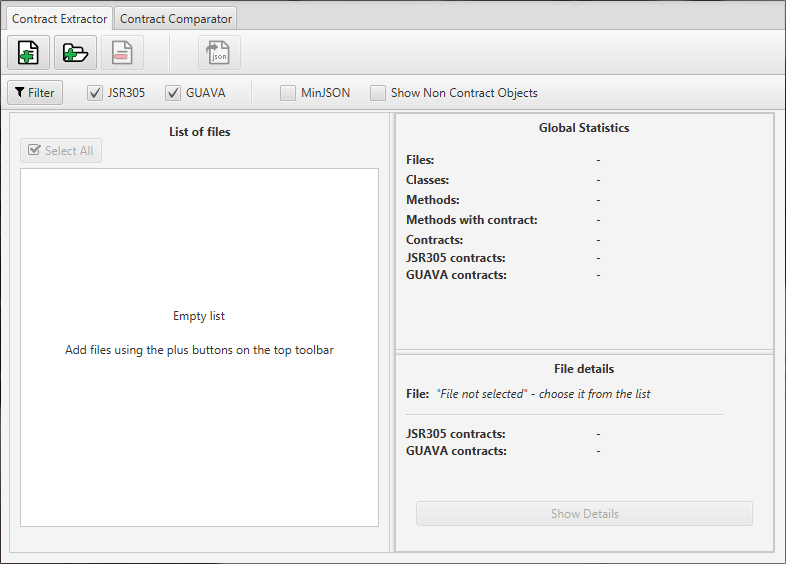
\includegraphics[width=1\textwidth]{img/guide01.png}
					\caption[guide01]{Výchozí stav uživatelské aplikace}
					\label{guide01}
				\endminipage\hfill
			\end{figure}
			
			\subsubsection{Extrakce kontraktů - základní zobrazení}
			
				\paragraph{Tlačítka pro přidání souborů}				
					Pod záložkami je panel nástrojů. Pomocí něj je možné soubory přidávat, odebírat či exportovat. První tlačítko (zelené plus na ikoně souboru) slouží k přidání individuálních souborů. Po jeho stisknutí se zobrazí okno pro výběr souborů. Je možné vybrat jeden či více souborů, ale pouze ty, které mají koncovku \texttt{.java} nebo \texttt{.class}. Pomocí druhého tlačítka (zelené plus na ikoně složky) je možné vybrat adresář a přidat tak všechny zdrojové či přeložené Java soubory z daného adresáře.\\
			
				\paragraph{Přidání souborů}
					Po přidání souborů jedním z těchto způsobů se vybrané položky zobrazí v seznamu v levé části okna, jak je vidět na obrázku \ref{guide02}. Přidání souborů může nějakou dobu trvat, protože jsou v této fázi všechny soubory zároveň analyzovány a jsou z nich extrahovány kontrakty. Doba této operace závisí na počtu i komplexnosti souborů a také na výkonu zařízení. Pokud jsou přidány i soubory, které kontrakty neobsahují, v seznamu se nezobrazí. To se dá změnit nastavením filtrů (viz níže).\\
			
			\begin{figure}[!htb]
				\minipage{1\textwidth}	
					\centering
					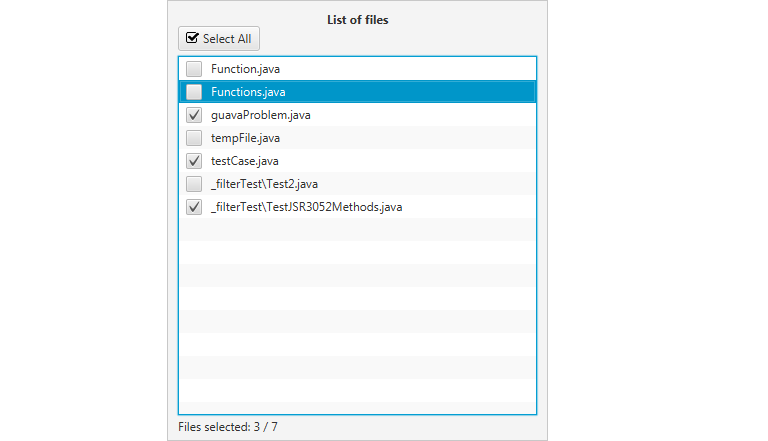
\includegraphics[width=1\textwidth]{img/guide02.png}
					\caption[guide02]{Extrakce kontraktů - seznam aktuálních souborů}
					\label{guide02}
				\endminipage\hfill
			\end{figure}			
			
				\paragraph{Odebírání a označování souborů}
					Třetí tlačítko na panelu (červené mínus na ikoně souboru) slouží k odebírání souborů. Z obrázku \ref{guide02} je patrné, že každý souboru v seznamu má po své levé straně zaškrtávací pole. Po jeho vybrání je soubor označen a následně je možné jej pomocí tlačítka pro odebrání smazat se seznamu (fyzický soubor zůstane nedotčen). Ve spodní částí oblasti se seznamem je zobrazen počet vybraných souborů z celkového počtu souborů v seznamu. Pomocí tlačítka \textbf{Select All} je také možné vybrat všechny soubory najednou (pokud již jsou všechny vybrány, tlačítko změní popisek na \textbf{Deselect All} a naopak zruší celý výběr).\\
			
				\paragraph{Export souborů}
					Posledním tlačítkem je export souborů. Po jeho stisknutí se zobrazí okno, kde se zvolí adresář, kam se mají exportovat všechny označené soubory. Výsledkem je soubor typu JSON pro každý z vybraných souborů. Zároveň je vytvořen jeden soubor \texttt{\_globalStatistics.json}, kde jsou uloženy globální statistiky o daných souborech. Podobu jednotlivých souborů ve formátu JSON je možné také vidět v detailech jednotlivých souborů (viz níže).\\
			
				\paragraph{Globální statistiky}
					Nahoře, v pravé části okna, je sekce \textbf{Global Statistics}, kde jsou zobrazeny globální statistiky pro všechny soubory v seznamu (jedná se o stejné informace, které jsou exportovány do speciálního souboru). Je zde informace o celkovém počtu souborů (\textbf{Files}), o počtu tříd (\textbf{Classes}) a počtu metod (\textbf{Methods}). Také je zde počet metod s kontrakty (\textbf{Methods with contracts}) a také počet samotných kontraktů (\textbf{Contracts}). Poslední informací je počet kontraktů pro jednotlivé typy reprezentací (např. \textbf{JSR305 contracts}). Tyto globální statistiky je možné vidět na obrázku \ref{guide03}.
			
			\begin{figure}[!htb]
				\minipage{1\textwidth}	
					\centering
					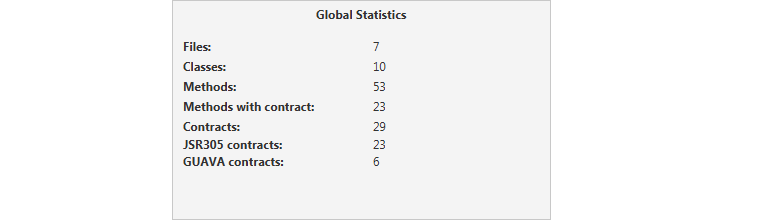
\includegraphics[width=1\textwidth]{img/guide03.png}
					\caption[guide03]{Extrakce kontraktů - Globální statistiky}
					\label{guide03}
				\endminipage\hfill
			\end{figure}
			
				\paragraph{Sekce s detaily souboru}
					Pod globálními statistikami se nachází panel s detaily o aktuálně vybraném souboru (viz obrázek \ref{guide04}). Zde se nejedná o výběr pomocí zaškrtávací pole, ale označení souboru kliknutím na jeho název (nebo jinam do oblasti daného řádku). Označený soubor je vidět na obrázku \ref{guide02}, kde je modře zvýrazněn (soubor \texttt{Functions.java}). Tyto detaily zobrazují absolutní cestu k danému souboru a také počet jednotlivých reprezentací kontraktů, které se v daném souboru nacházejí. Také je zde tlačítko \textbf{Show Details}, pomocí kterého je možné zobrazit okno s podrobnostmi o daném souboru (viz níže).\\
			
				\paragraph{Filtry}					
					Poslední sekcí extrakční části jsou filtry, které jsou zobrazeny pod panelem nástrojů a jsou realizovány zaškrtávacími políčky (viz obrázek \ref{guide01}). Pomocí těchto filtrů je možné změnit zobrazení dat v aplikaci a také ovlivnit export. Nejprve jsou zde jednotlivé reprezentace kontraktů, které je možné libovolně zobrazovat či skrývat (ve výchozím stavu jsou všechny viditelné). Pak je zde možnost \textbf{Show Non Contract Objects}. Ta určuje, zda se mají zobrazovat i soubory, třídy či metody, které neobsahují žádný kontrakt.\\
						
			Posledním filtrem je \textbf{MinJSON}. Pokud je tento filtr použit, veškerý export je ukládán v minimalizovaném formátu JSON. To může být užitečné např. při další práci s těmito soubory, aby se zmenšila jejich velikost. Ve výchozím stavu je tento přepínač vypnutý a všechny exporty jsou prováděny v~tzv. \emph{pretty print}, což znamená, že je JSON dobře čitelný pro člověka, protože je členěn dle hierarchie.\\
			
			Aby nastavené filtry byly aktivovány, je třeba stisknout tlačítko \textbf{Filter}. Kromě filtru \textbf{MinJSON}, který ovlivní pouze export, ovlivňují filtry vše v~aplikaci. Mění tedy seznam souborů, statistiky i detail daného souboru.
			
			\begin{figure}[!htb]
				\minipage{1\textwidth}	
					\centering
					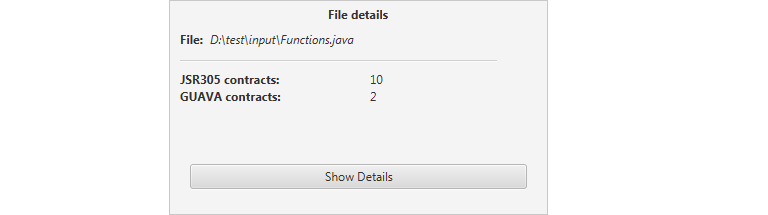
\includegraphics[width=1\textwidth]{img/guide04.png}
					\caption[guide04]{Extrakce kontraktů - sekce detailu souboru}
					\label{guide04}
				\endminipage\hfill
			\end{figure}
			
				\paragraph{Aplikace po extrakci kontraktů}
					Na obrázku \ref{guide09} je možné vidět, jak aplikace vypadá jako celek ve chvíli, kdy byly přidány soubory.
					
			\begin{figure}[!htb]
				\minipage{1\textwidth}	
					\centering
					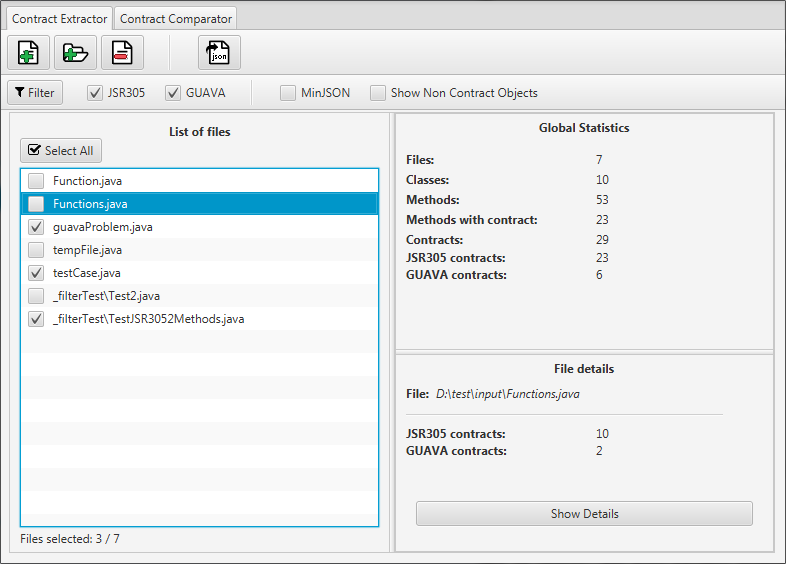
\includegraphics[width=1\textwidth]{img/guide09.png}
					\caption[guide09]{Aplikace po extrakci kontraktů}
					\label{guide09}
				\endminipage\hfill
			\end{figure}						
			
			\subsubsection{Extrakce kontraktů - detail souboru}
				Po stisku tlačítka \textbf{Show Details} se zobrazí nové okno s podrobnostmi o~vybraném souboru (viz \ref{guide05}). Je zde tedy název souboru a statistické údaje jako je počet tříd, metod a kontraktů. Cennou informací je zde strom zpracovaného souboru. Zde jsou vidět jednotlivé třídy a metody daného souboru v hierarchické podobě a uvnitř nich se nachází samotné kontrakty. Zde je možné zjistit podrobnosti o tom, o jaké kontrakty se jedná, jaký mají přesný tvar atd. Tento strom je zjednodušenou verzí JSON verze tohoto souboru. Ten je možné zobrazit přepnutím záložky z \textbf{Tree View} do \textbf{Raw Unfiltered JSON}. Jedná se o stejná data, která jsou uložena v případě využití exportu.\\
				
				Kromě zobrazení těchto informací zde není možné provádět žádnou aktivní činnost, okno je možné pouze zavřít standardním způsobem. Okno se také zavře v případě, že byla zavřena hlavní aplikace, nicméně je možné mít otevřené libovolné množství těchto oken s podrobnostmi, což je možné využít např. při jejich porovnávání.
				
			\begin{figure}[!htb]
				\minipage{1\textwidth}	
					\centering
					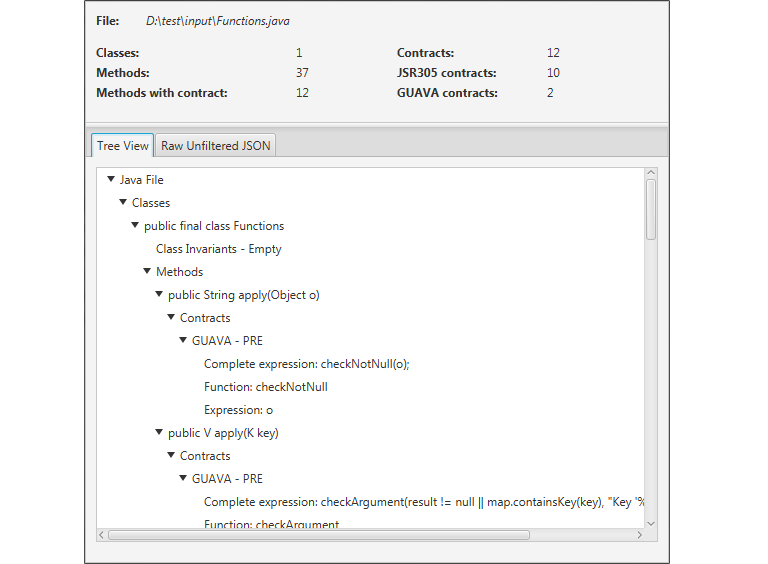
\includegraphics[width=1\textwidth]{img/guide05.png}
					\caption[guide05]{Extrakce kontraktů - Okno s detaily souboru}
					\label{guide05}
				\endminipage\hfill
			\end{figure}
			
	
	\subsubsection{Porovnávání kontraktů - základní zobrazení}
		Jak již bylo zmíněno výše, aby bylo možné porovnávat kontrakty je třeba přepnout záložku na vrcholu okna na \textbf{Contract Comparator}. Tím se změní rozložení aplikace, jak je vidět na obrázku \ref{guide06}. Jediné co je mezi oběma částmi sdíleno, je nastavení společných filtrů. Nicméně obě části aplikace jsou si velmi podobné, a proto zde budou rozepsány pouze ty informace, které se liší oproti extrakční části.
		
			\begin{figure}[!htb]
				\minipage{1\textwidth}	
					\centering
					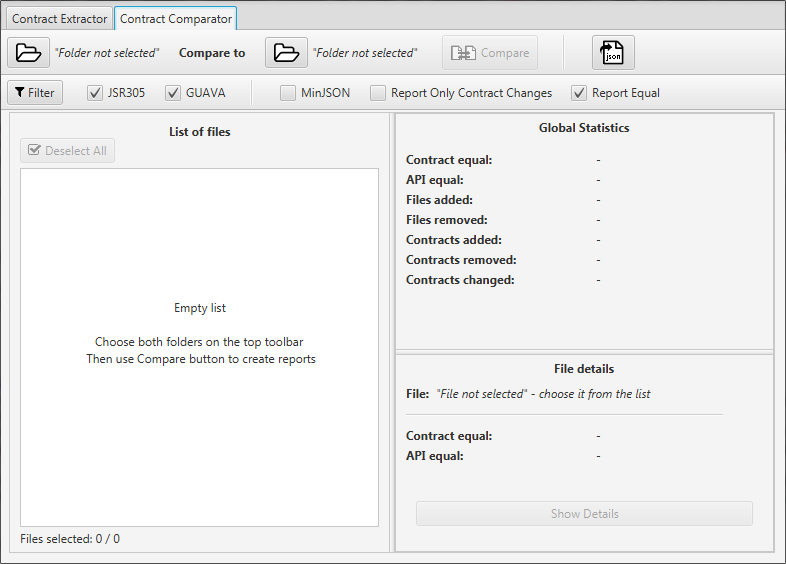
\includegraphics[width=1\textwidth]{img/guide06.png}
					\caption[guide06]{Výchozí stav porovnávací části aplikace}
					\label{guide06}
				\endminipage\hfill
			\end{figure}
		
		\paragraph{Panel nástrojů}	
			Aplikace umožňuje pouze porovnání dvou složek. Tyto složky vybereme pomocí panelu nástrojů, který je oproti extrakční části změněn. První dvě tlačítka slouží tedy k výběru složek, po jejich stisknutí se zobrazí okno průzkumníka souborů, kde je možné vybrat pouze adresář. Tyto vybrané složky pak můžeme porovnat pomocí tlačítka \textbf{Compare}, které se po výběru složek zpřístupní. Tímto se podobně jako v předchozí části přidají soubory do seznamu v levé části. Tato akce opět zabere nějaký čas, během kterého je zobrazeno načítací okno. V případě, že bychom chtěli porovnat jiné složky, stačí zvolit novou složku pomocí jednoho z tlačítek a~aplikace smaže všechny ostatní hodnoty. Na rozdíl od části pro extrakci zde není možné soubory mazat, ale vybrané soubory je možné extrahovat opět pomocí tlačítka na konci panelu. Nicméně zde není možné vybrat, které soubory chceme exportovat, ale automaticky se exportují všechny. Důvodem tohoto chování je, že se jedná o porovnání dvou složek, jehož součástí jsou všechny porovnání daných souborů. Nejsou to nezávislé položky jako v případě extrakce.\\
		
		\paragraph{Seznam souborů}
			Seznam souborů vypadá stejně jako v extrakční části. Rozdílem však je, že zde jednotlivé položky představují zprávy o porovnání daných souborů. Každá tato zpráva pak obsahuje hierarchii tříd a metod, kde je pro každý kontrakt informace, zda byl přidán odebrán či změněn. Také jsou zde informace o přidaných a odebraných metodách a shrnutí zda je daný soubor se svým protějškem shodný v rámci API a kontraktů. Velkým rozdílem je to, že jednotlivé položky není možné označovat. Vzhledem k~tomu, že soubory nelze mazat ani jednotlivě exportovat, není to třeba.
		
		\paragraph{Globální statistiky}
			Zbytek aplikace funguje stejným způsobem jako část pro extrahování, ale zobrazená data se liší. Globální statistiky zobrazují hodnoty z porovnání obou složek. Je zde informace o tom, zda jsou dané adresáře shodné na úrovni kontraktů (\textbf{Contract equal}) či na úrovni API (\textbf{API equal}). Je zde také informace o tom, kolik souborů bylo oproti předchozí složce přidáno respektive odebráno (\textbf{Files added / removed}). Tyto informace jsou zde také pro kontrakty. Přibývá však i informace o počtu změněných kontraktech (\textbf{Contracts added / removed / changed}).\\
		
		\paragraph{Detail souboru}
			Sekce zobrazující detaily o souboru obsahují mimo jména souboru také informaci o tom, zda je tento soubor shodný v rámci API a~kontraktů vůči svému protějšku. Jedná se tedy o informace, které jsou v~globálních statistikách, zde se však týkají pouze vybraného souboru. Také je zde tlačítko \textbf{Show Details}, které zobrazí okno s detaily o daném porovnání.\\
				
		\paragraph{Filtry}
			I v této části jsou filtry umožňující skrýt různé reprezentace kontraktů a také je tu filtr pro minimalistický formát exportu. Navíc zde však přibyl filtr \textbf{Report Only Contract Changes}. Pokud je označen, nejsou zobrazeny žádné informace o souborech, třídách a metodách, které nijak neovlivňují kontrakty. To může velmi zjednodušit data, pokud nás zajímají pouze informace  kontraktech.\\
			
			Posledním filtrem je \textbf{Report Equal}. Ve své výchozí pozici je zapnutý a určuje to, zda se mají zobrazovat i zprávy o tom, že jsou dané soubory, třídy, metody a kontrakty shodné. Vypnutím tohoto filtru můžeme snadno pouze změny a shodné objekty ignorovat.\\
		
		\paragraph{Aplikace po porovnání složek}	
			Na obrázku \ref{guide08} je zachycen stav aplikace po porovnání dvou složek. Jak je vidět, tlačítko \textbf{Compare} není momentálně přístupné. Znovu se zpřístupní ve chvíli, kdy se vybere nová složka, důvodem je, že opětovné porovnání stejných složek by bylo zbytečné.
			
			\begin{figure}[!htb]
				\minipage{1\textwidth}	
					\centering
					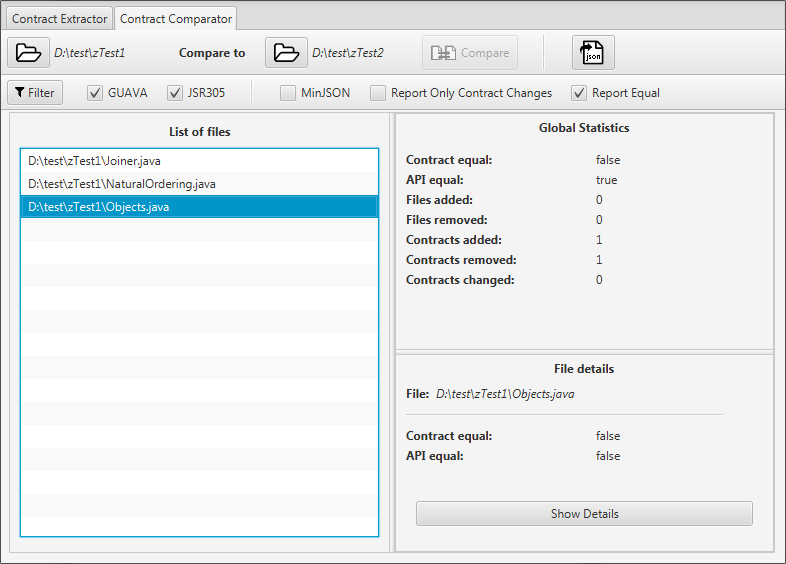
\includegraphics[width=1\textwidth]{img/guide08.png}
					\caption[guide08]{Stav aplikace po porovnání vybraných složek}
					\label{guide08}
				\endminipage\hfill
			\end{figure}			
			
	\subsubsection{Porovnávání kontraktů - detail souboru}
		Po stisku tlačítka \textbf{Show Details} se opět otevře nové okno s podrobnostmi o~dané položce (viz \ref{guide07}). Stejně jako v případě extrakce, jsou zde také v horní části statistické informace a dole je poté stromové zobrazení. Co se statistických údajů týče, jsou zde informace o tom, zda je daný soubor shodný v~rámci kontraktů a API se svým protějškem. Také jsou zde informace o tom, kolik tříd, metod a kontraktů se přidalo nebo ubralo. V případě kontraktů pak také kolik se jich změnilo.\\
		
		Stromové zobrazení je opět možné přepnout na JSON formát. Provede se to přepnutím záložky z \textbf{Tree View} na \textbf{Raw Unfiltered JSON}. Jedná se o~stejný JSON, který je exportován pokud není vybraná možnost \textbf{MinJSON}.
		
			\begin{figure}[!htb]
				\minipage{1\textwidth}	
					\centering
					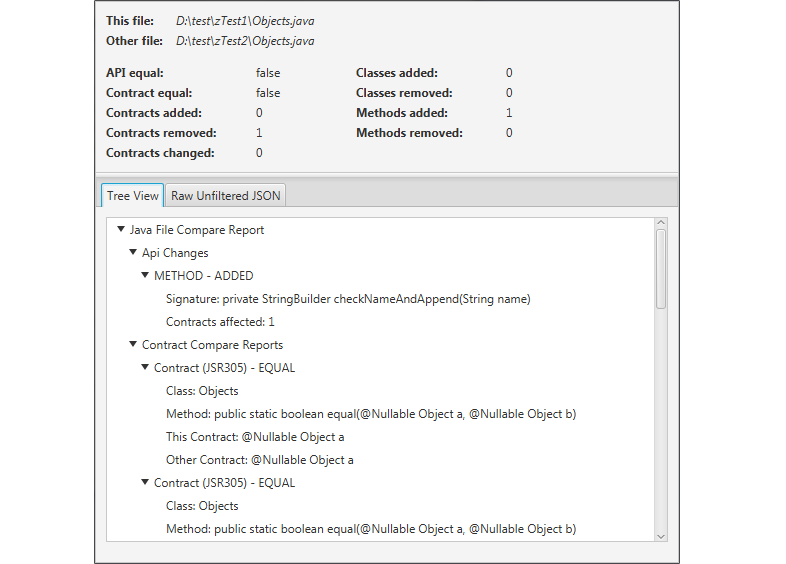
\includegraphics[width=1\textwidth]{img/guide07.png}
					\caption[guide07]{Porovnávání kontraktů - Okno s detaily souboru}
					\label{guide07}
				\endminipage\hfill
			\end{figure}		
		
	\subsection{Konzolová část}
		Pokud nepotřebujeme grafické rozhraní je možné použít konzolovou část aplikace. Pokud aplikaci spustíme se správnými parametry jednorázově provede extrakci kontraktů z dané složky či porovnání dvou složek. Výsledek je pak exportován ve formátu JSON do zvoleného adresáře. Dále je popsán způsob jakým je třeba zadat parametry.\\
		
		Jako první parametr musí být vždy uveden \texttt{-e} pro extrakci kontraktů nebo \texttt{-c} pro porovnávání složek. Speciálním případem je pak parametr \texttt{-h}, který zobrazí nápovědu (je možné použít i \texttt{---help)}.
		
		\subsubsection{Extrakce kontraktů}
			Příkaz pro extrahování kontraktů má tento tvar:\\\\
			\- \- \- \texttt{-e <input\_folder> <output\_folder> [-r] [-m]}\\
			
			Jak již bylo zmíněno, parametr \texttt{-e} značí, že se jedná o extrakci kontraktů. \texttt{<input\_folder>} je povinný parametr, kde je třeba uvést složku, ze které budou kontrakty extrahovány. Dalším povinným parametrem je \texttt{<output\_folder>}, kde je třeba uvést výstupní složku, kam se uloží exportovaná data.\\
			
			Volitelný parametr \texttt{-r} určuje, zda mají být odebrány soubory, třídy či metody, které neobsahují žádné kontrakty. Export spuštěný s tímto parametrem bude tedy stručnější a bude obsahovat pouze objekty, které obsahují kontrakty.\\
			
			Druhým a posledním volitelným parametrem je \texttt{-m}. Pomocí něj můžeme zajistit, že výstupní JSON bude ve své minimalistické podobě.\\
			
			Zde je příklad spuštění aplikace tak, aby extrahovala všechny kontrakty ze složky \texttt{data/project} do \texttt{my/output} v minimalistickém formátu:\\\\
			\- \- \- \texttt{java -jar ContractMnager.jar -e data/project my/output -m}
			
		\subsubsection{Porovnávání kontraktů}
			Příkaz pro porovnávání kontraktů má tento tvar:\\\\
			\- \- \- \texttt{-c <input\_folder1> <input\_folder2> <output\_folder> [-q] [-o] [-m]}\\
			
			Zde je třeba začít pomocí \texttt{-c}, což značí porovnávání. Následují tři povinné parametry, kde prvním (\texttt{<input\_folder1>}) a druhým (\texttt{<input\_folder2>}) jsou vstupní složky, jejichž obsah má být porovnán z hlediska API a zejména z hlediska rozdílnosti kontraktů. Třetím povinným parametrem je opět výstupní složka (\texttt{<output\_folder>}), kam mají být exportovány výsledky.\\
			
			Porovnání kontraktů má tři volitelné parametry, které korespondují s~grafickou částí aplikace. Prvním z nich je \texttt{-q}. Ten určuje, zda mají být exportovány také objekty, které byly vyhodnoceny jako shodné. Ve výchozím stavu jsou tedy tato data ignorována.\\
			
			Dalším parametrem je \texttt{-o}. Pokud je tento přepínač vybrán, budou exportovány pouze změny, které se přímo týkají kontraktů. Tímto je možné zanedbat změny API, které se přímo kontraktů netýkají.\\
			
			Posledním volitelným parametrem je opět \texttt{-m}, který i jako v předchozím případě umožňuje minimalistickou verzi formátu JSON.